\documentclass[11pt,a4paper]{article}
\usepackage[T1]{fontenc}
\usepackage[utf8]{inputenc}
\usepackage[french]{babel}
\usepackage{lmodern,microtype}
\usepackage[a4paper,margin=2.5cm]{geometry}
\usepackage{amsmath,amssymb,booktabs,tabularx,graphicx,float,caption,subcaption}
\usepackage{xcolor,hyperref}
\usepackage[backend=biber,style=authoryear,sorting=nyt,maxbibnames=99]{biblatex}
\addbibresource{references.bib}
\definecolor{paperblue}{HTML}{153A5B}
\hypersetup{colorlinks=true,linkcolor=paperblue,citecolor=paperblue,urlcolor=paperblue}
\captionsetup{font=small,labelfont=bf}

\title{\textbf{Estimation et dynamique des distributions risque-neutre à partir d'options SPX}\\[0.4em]
\large Projet PI\textsuperscript{2} n\textsuperscript{o} 176 — Premier rapport de recherche}
\author{Rayan Ait Arkoub \and Matthieu Balliste \and Ilan Chahdi \and Nathan Denoux \and Jordi Paris\\
\small ESILV — Pôle Léonard de Vinci\\
\small Tuteur : Matthieu Garcin}
\date{20 octobre 2026}

\begin{document}
\maketitle

\begin{abstract}
Nous développons un pipeline reproductible d'estimation de distributions risque-neutre
(RND) à partir d'options sur l'indice S\&P 500. Une photographie différée de Cboe du
16 octobre 2026 est nettoyée, puis le forward et le facteur d'actualisation sont estimés
par parité call-put. Une paramétrisation SVI à cinq paramètres fournit une coupe de
volatilité commune à l'ensemble des strikes. La densité est ensuite extraite par la
relation de Breeden--Litzenberger et calculée indépendamment en Python et en Julia.
Pour l'échéance à 91 jours, 338 observations alimentent la calibration, la RMSE de prix
vaut 1,144 point d'indice et la masse brute de densité atteint 0,9953 sur la grille.
Nous étendons l'exercice à six maturités comprises entre 31 et 182 jours et construisons
une surface tridimensionnelle des RND en log-moneyness. Cette surface décrit la structure
par terme à une date donnée ; l'étude dynamique temporelle nécessitera un historique
quotidien Bloomberg, OptionMetrics ou Cboe DataShop.
\end{abstract}

\noindent\textbf{Mots-clés :} distribution risque-neutre, options SPX, Breeden--Litzenberger,
SVI, volatilité implicite, structure par terme, Julia.\\
\textbf{Codes JEL :} C14, C58, G13, G17.

\section{Introduction}
Les prix d'options contiennent une information prospective sur la distribution du
sous-jacent à l'échéance. Dans Black--Scholes, cette distribution est lognormale et
une volatilité unique devrait expliquer tous les strikes. L'existence empirique du
smile invalide cette restriction. Une volatilité implicite peut ajuster chaque option
séparément, mais ne constitue pas un modèle commun parcimonieux de la chaîne.

Ce projet poursuit cinq objectifs : constituer une base historique, comparer trois
méthodes d'extraction de RND, mesurer leur stabilité, prévoir leur dynamique au moyen
d'un modèle factoriel et tester une application à la couverture. Le présent article
documente le premier jalon : une estimation complète sur SPX, sa validation Julia et
une extension tridimensionnelle selon la maturité.

\section{Revue de littérature}
\textcite{breeden_litzenberger_1978} relient les prix d'états à la dérivée seconde des
calls. \textcite{figlewski_2010} et \textcite{figlewski_2018} soulignent les difficultés
empiriques : bruit bid-ask, interpolation, support fini et queues. \textcite{cui_yu_2021}
proposent une alternative Fourier-cosinus reposant sur l'intégration plutôt que la
double dérivation. \textcite{avellaneda_et_al_2001} construisent une mesure calibrée
par minimisation d'entropie relative. Pour la dynamique, \textcite{giacomini_et_al_2009}
réduisent les densités en facteurs semiparamétriques, tandis que \textcite{taboga_2016}
étudie l'incertitude et le risque de multimodalité artificielle.

\section{Cadre théorique}
Sous la mesure risque-neutre $\mathbb{Q}$,
\begin{equation}
C_t(K,T)=D(t,T)\,\mathbb{E}^{\mathbb{Q}}_t[(S_T-K)^+].
\end{equation}
La relation de Breeden--Litzenberger est
\begin{equation}
q_t(K,T)=\frac{1}{D(t,T)}\frac{\partial^2 C_t(K,T)}{\partial K^2}.
\end{equation}
La parité call-put permet d'estimer simultanément le forward et l'actualisation :
\begin{equation}
C_t(K,T)-P_t(K,T)=D(t,T)[F_{t,T}-K].
\end{equation}

Pour lisser la coupe, nous utilisons la variance totale SVI brute
\begin{equation}
w(k)=a+b\left[\rho(k-m)+\sqrt{(k-m)^2+\sigma^2}\right],
\qquad k=\log(K/F).
\end{equation}
Cette étape fournit un modèle commun à cinq paramètres. Elle ne remplace pas
Breeden--Litzenberger : elle construit la fonction de prix régulière à dériver.

\section{Données}
La source est l'API publique différée de Cboe. La photographie principale est datée
du 16 octobre 2026 à 17:12:17. L'accès Bloomberg n'est pas disponible dans
l'environnement actuel. L'API publique ne fournit pas l'historique requis pour la
dynamique ; ce point constitue la principale dépendance externe.

\begin{table}[H]\centering
\caption{Échantillon principal SPX.}
\begin{tabular}{lr}\toprule
Spot & 7 682,18 \\
Échéance & 15 janvier 2027 \\
Maturité & 91 jours \\
Contrats avant filtrage & 1 446 \\
Cotations valides & 1 277 \\
Strikes call-put appariés & 362 \\
Points de calibration & 338 \\
\bottomrule\end{tabular}
\end{table}

\section{Méthodologie empirique}
Nous sélectionnons l'échéance la plus proche de l'horizon cible. Les cotations avec
bid nul, marché croisé, mid inférieur à 0,05 ou spread relatif supérieur à 35\,\%
sont écartées. Le mid est privilégié au dernier prix, dont l'horodatage sert seulement
de diagnostic. Une régression pondérée de la parité autour de la monnaie estime $F$
et $D$. Les calls OTM sont utilisés au-dessus du forward ; sous le forward, les puts
OTM sont transformés en calls synthétiques. Les volatilités implicites sont calibrées
par SVI, les calls reconstruits sur 1 601 strikes et la dérivée seconde calculée.

\begin{figure}[H]\centering
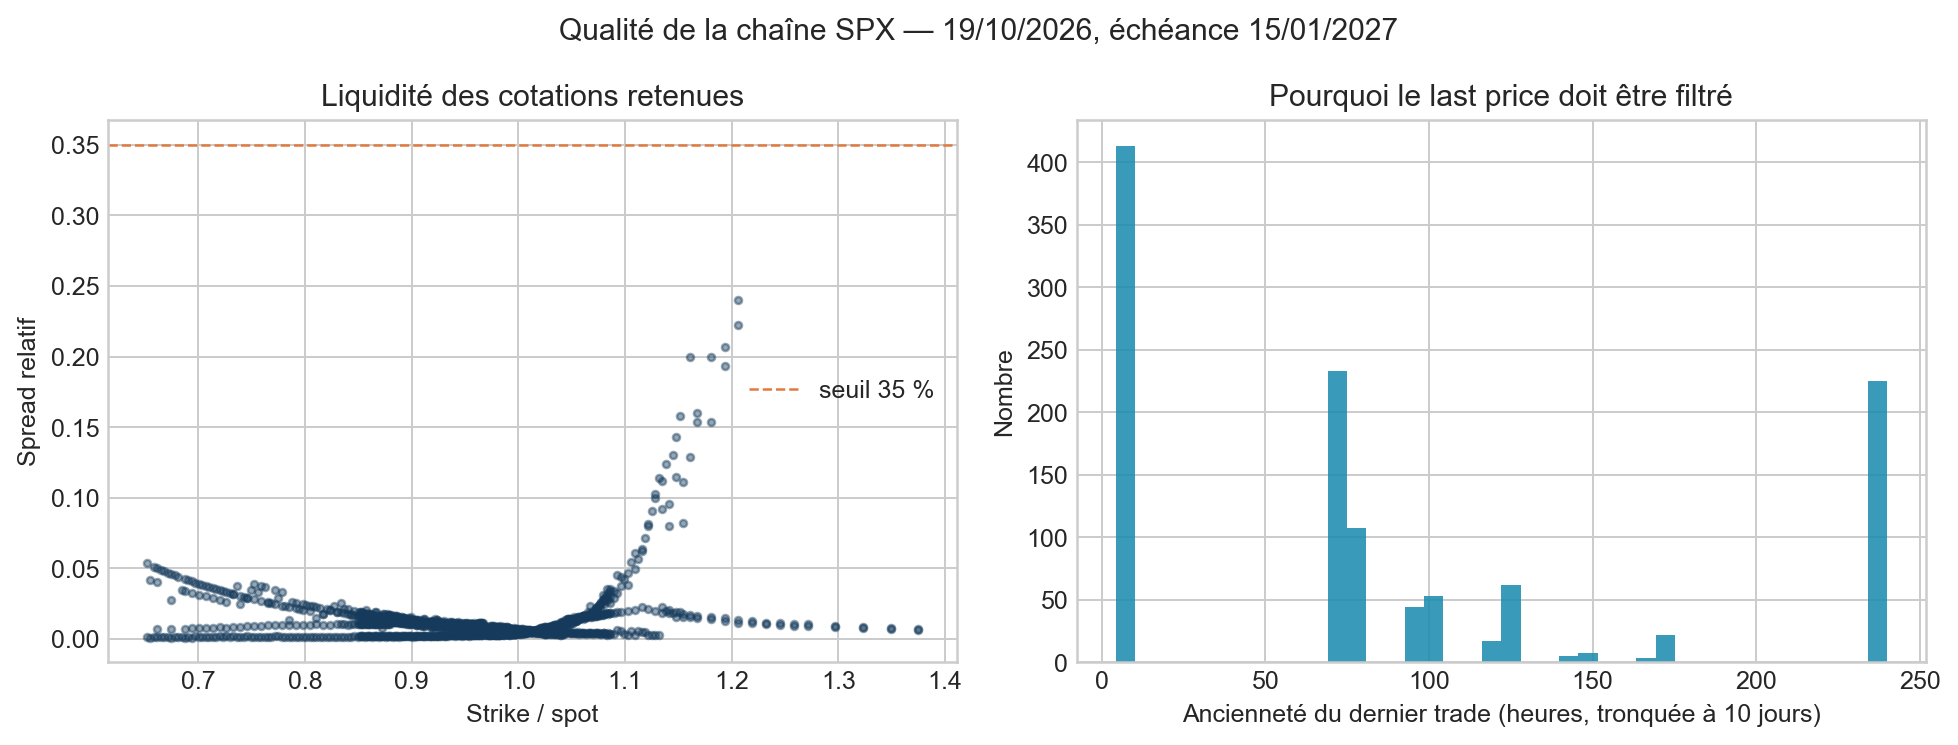
\includegraphics[width=0.94\textwidth]{results/01_data_quality.png}
\caption{Spreads relatifs et ancienneté des derniers échanges.}
\end{figure}

\section{Résultats pour l'échéance à 91 jours}
La parité fournit $F=7\,755{,}89$, $D=0{,}98837$ et un taux continu implicite de
4,69\,\%. La RMSE de parité est 0,118 point. Les paramètres SVI sont
$a=-0{,}02923$, $b=0{,}12073$, $\rho=-0{,}05133$, $m=0{,}08167$ et
$\sigma=0{,}26829$. La RMSE de prix atteint 1,144 point.

\begin{figure}[H]\centering
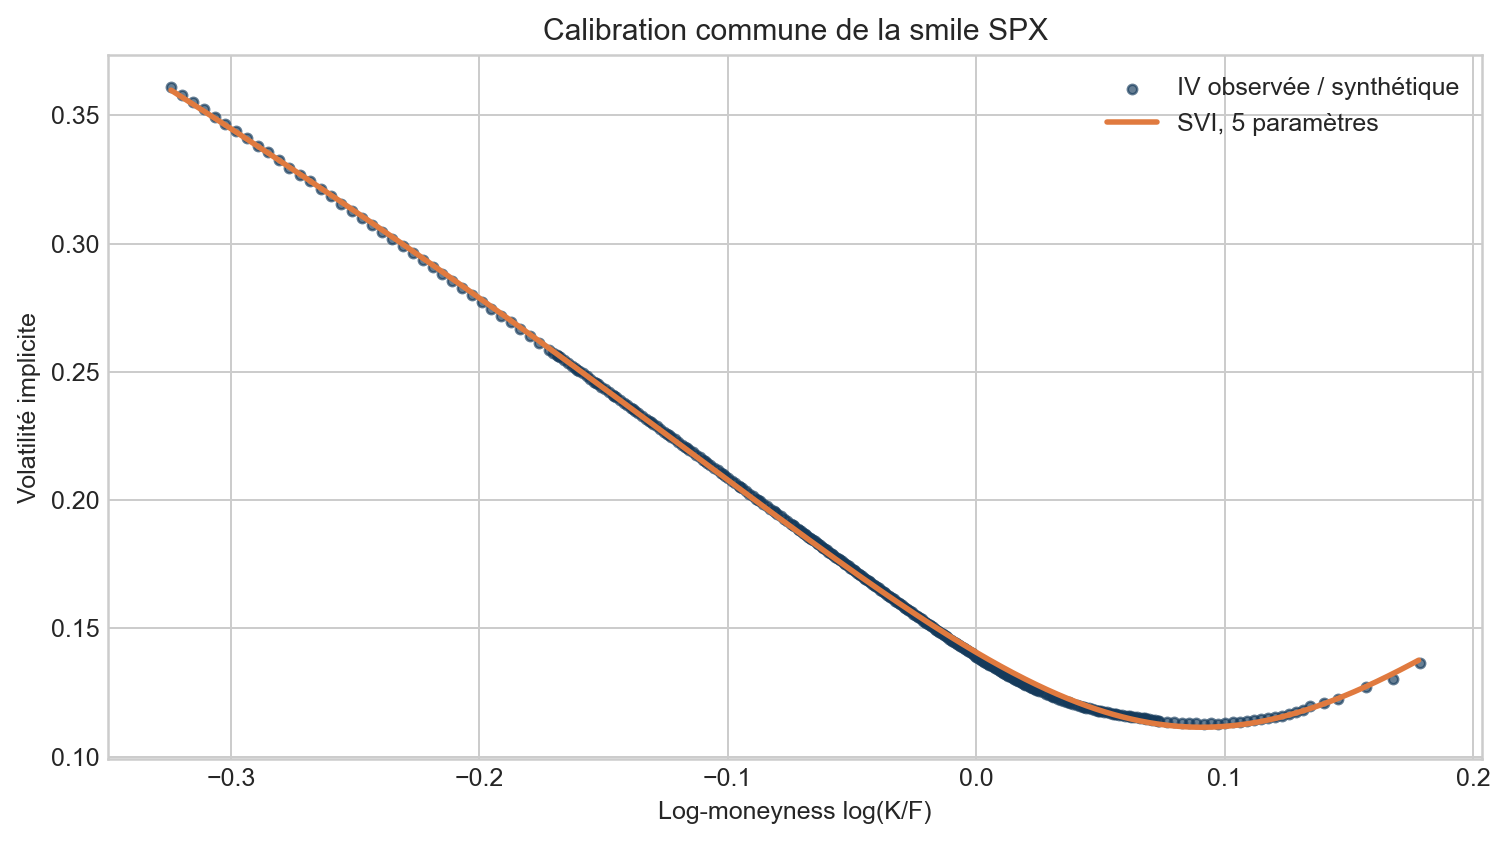
\includegraphics[width=0.82\textwidth]{results/02_svi_smile.png}
\caption{Smile observée et calibration commune SVI.}
\end{figure}

\begin{figure}[H]\centering
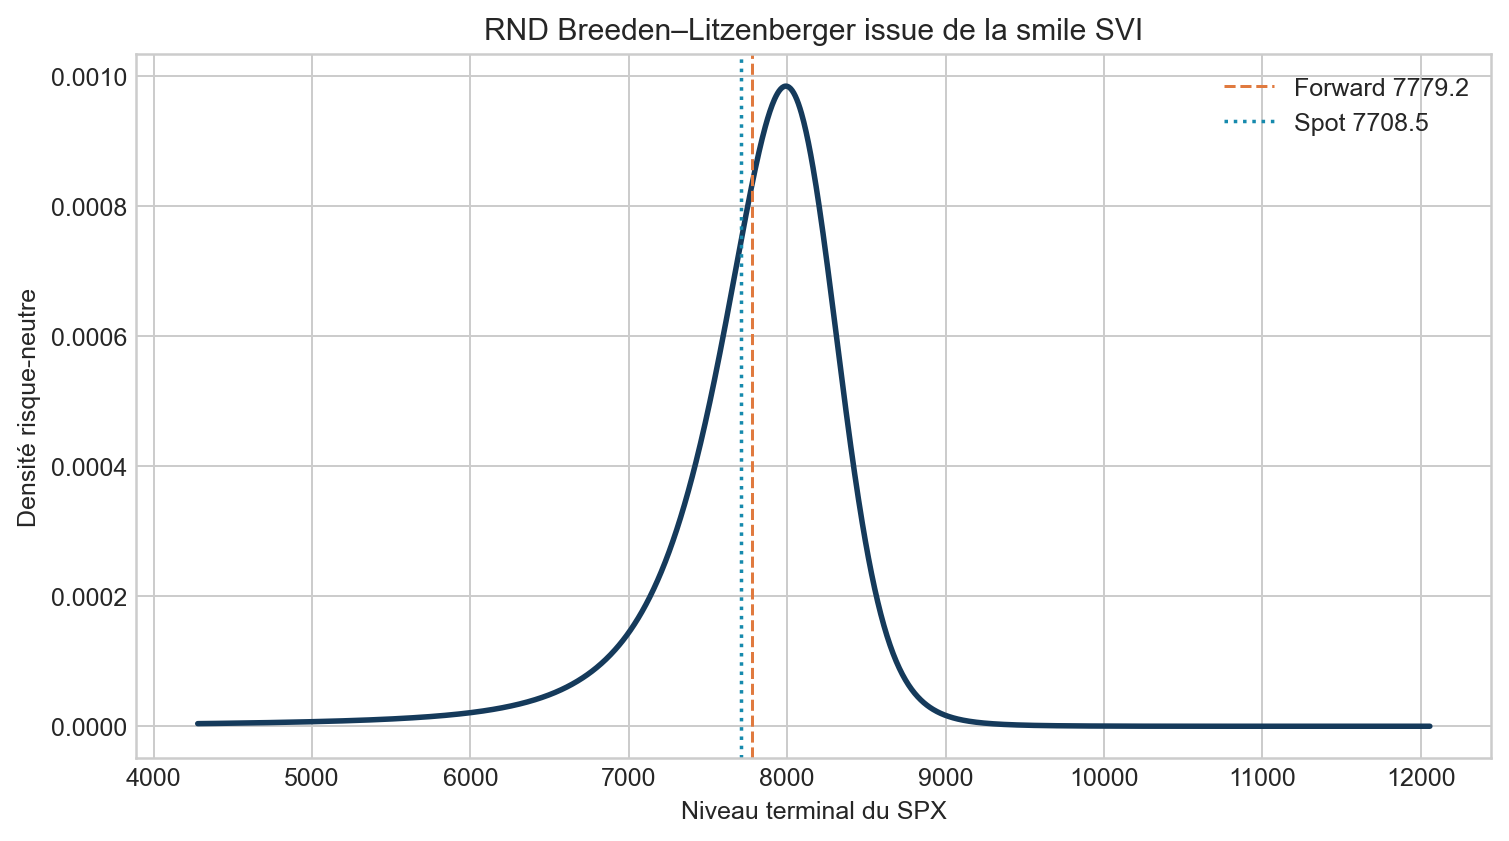
\includegraphics[width=0.82\textwidth]{results/04_risk_neutral_density.png}
\caption{RND obtenue par Breeden--Litzenberger.}
\end{figure}

La masse brute vaut 0,99528 et la masse négative absolue seulement 0,000117. Des
valeurs faiblement négatives apparaissent dans l'extrême queue droite, mais aucune
n'excède 0,1\,\% du pic en amplitude. Après troncature et normalisation, la moyenne
vaut 7 776,20. Ces écarts proviennent du support fini et de l'extrapolation SVI ; ils
motivent une future calibration eSSVI ou un lissage directement convexe.

\section{Structure tridimensionnelle des RND}
Nous répétons le pipeline sur six maturités : 31, 63, 91, 126, 154 et 182 jours.
Pour rendre les distributions comparables, elles sont exprimées en log-moneyness.
La densité transformée est
\begin{equation}
q_k(k)=q_S(F e^k)F e^k.
\end{equation}

\begin{figure}[H]\centering
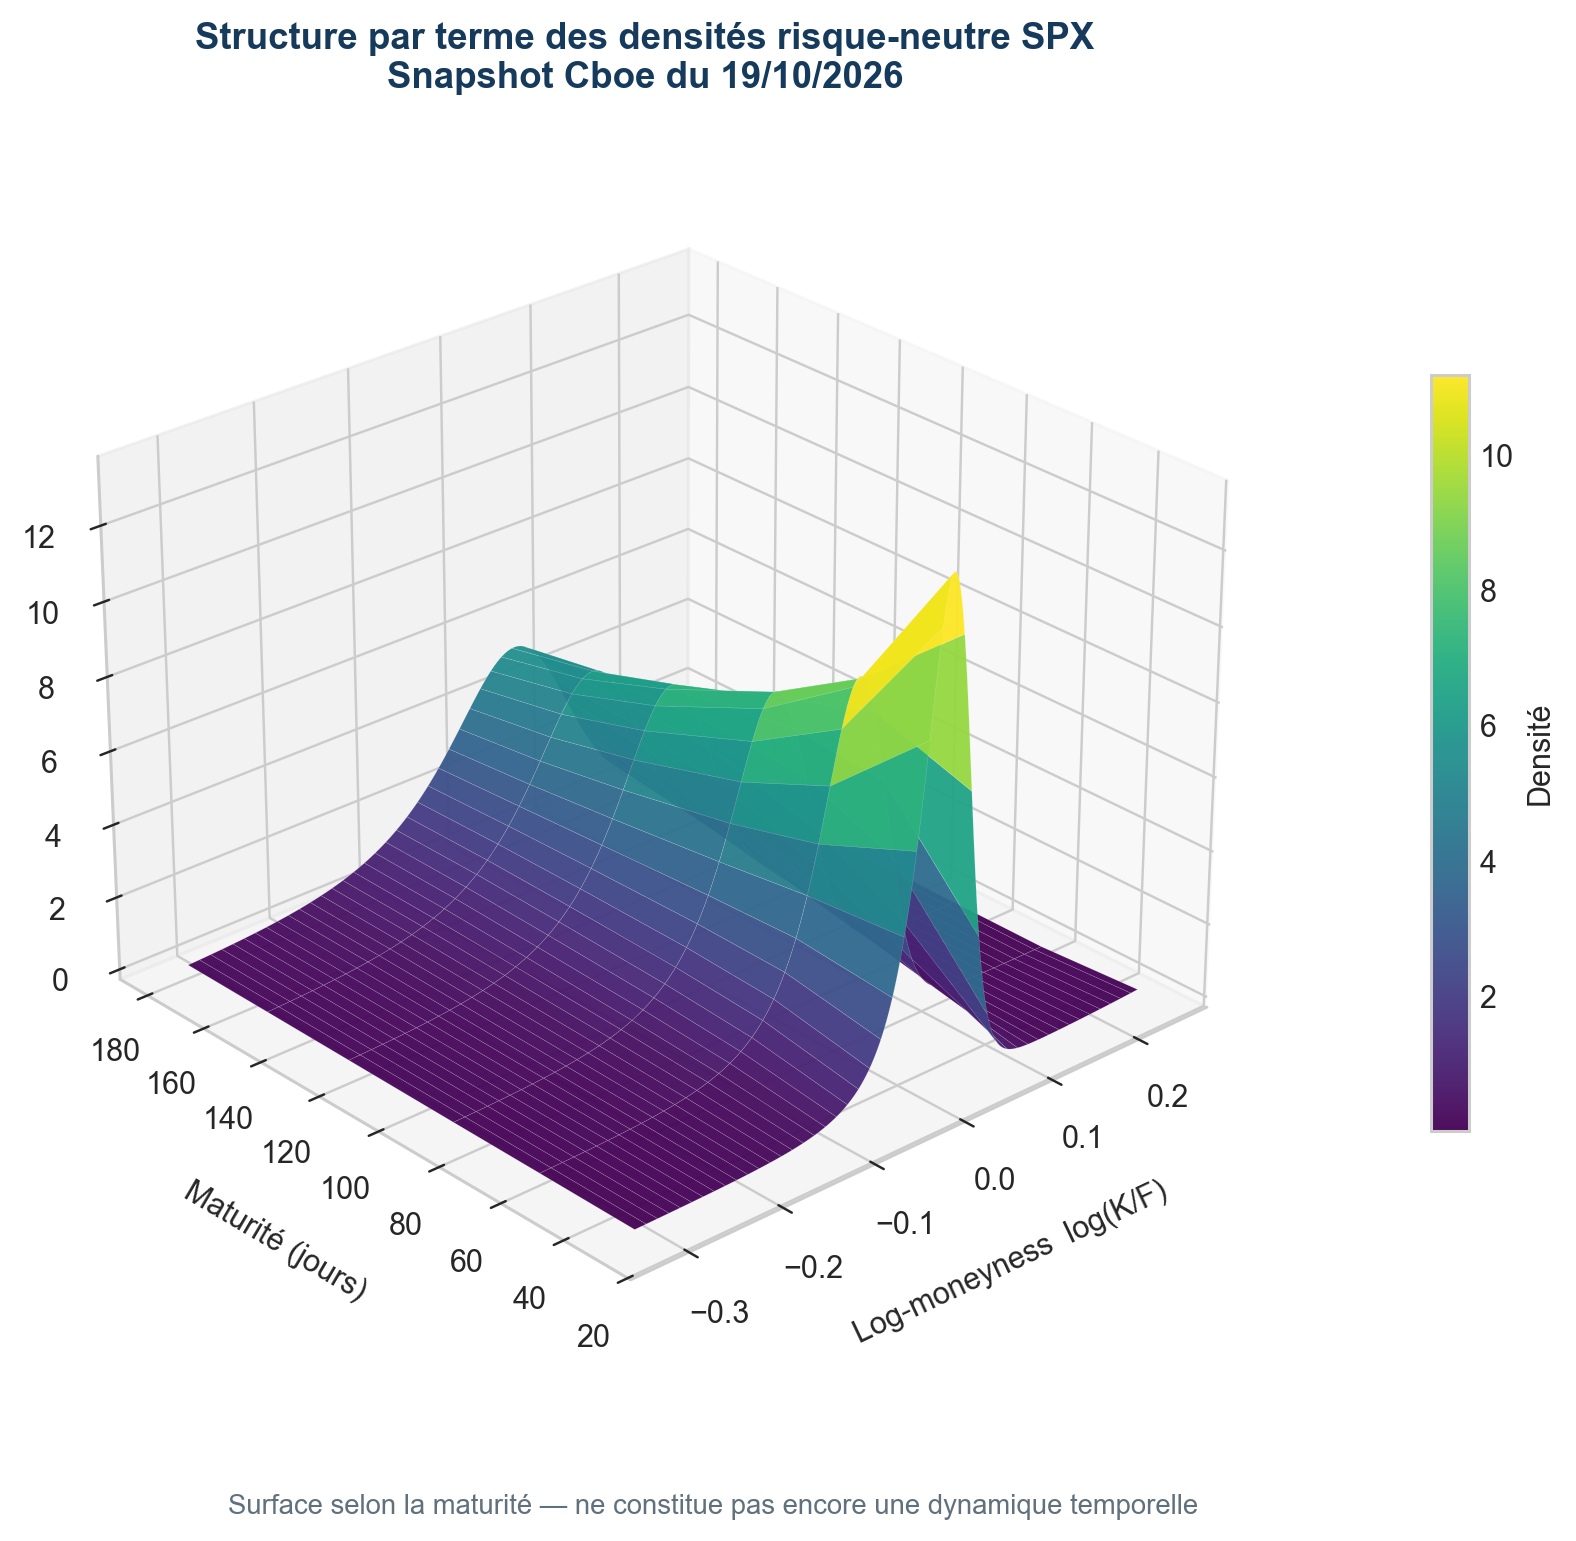
\includegraphics[width=\textwidth]{results/05_rnd_surface_3d_maturity.png}
\caption{Surface 3D des RND selon la maturité. Il s'agit d'une structure par terme
à date fixe, non d'une dynamique temporelle.}
\end{figure}

La surface montre une densité très concentrée à court terme, puis un aplatissement et
un élargissement progressifs avec la maturité. La carte thermique facilite la lecture
de la position du mode et de l'asymétrie.

\begin{figure}[H]\centering
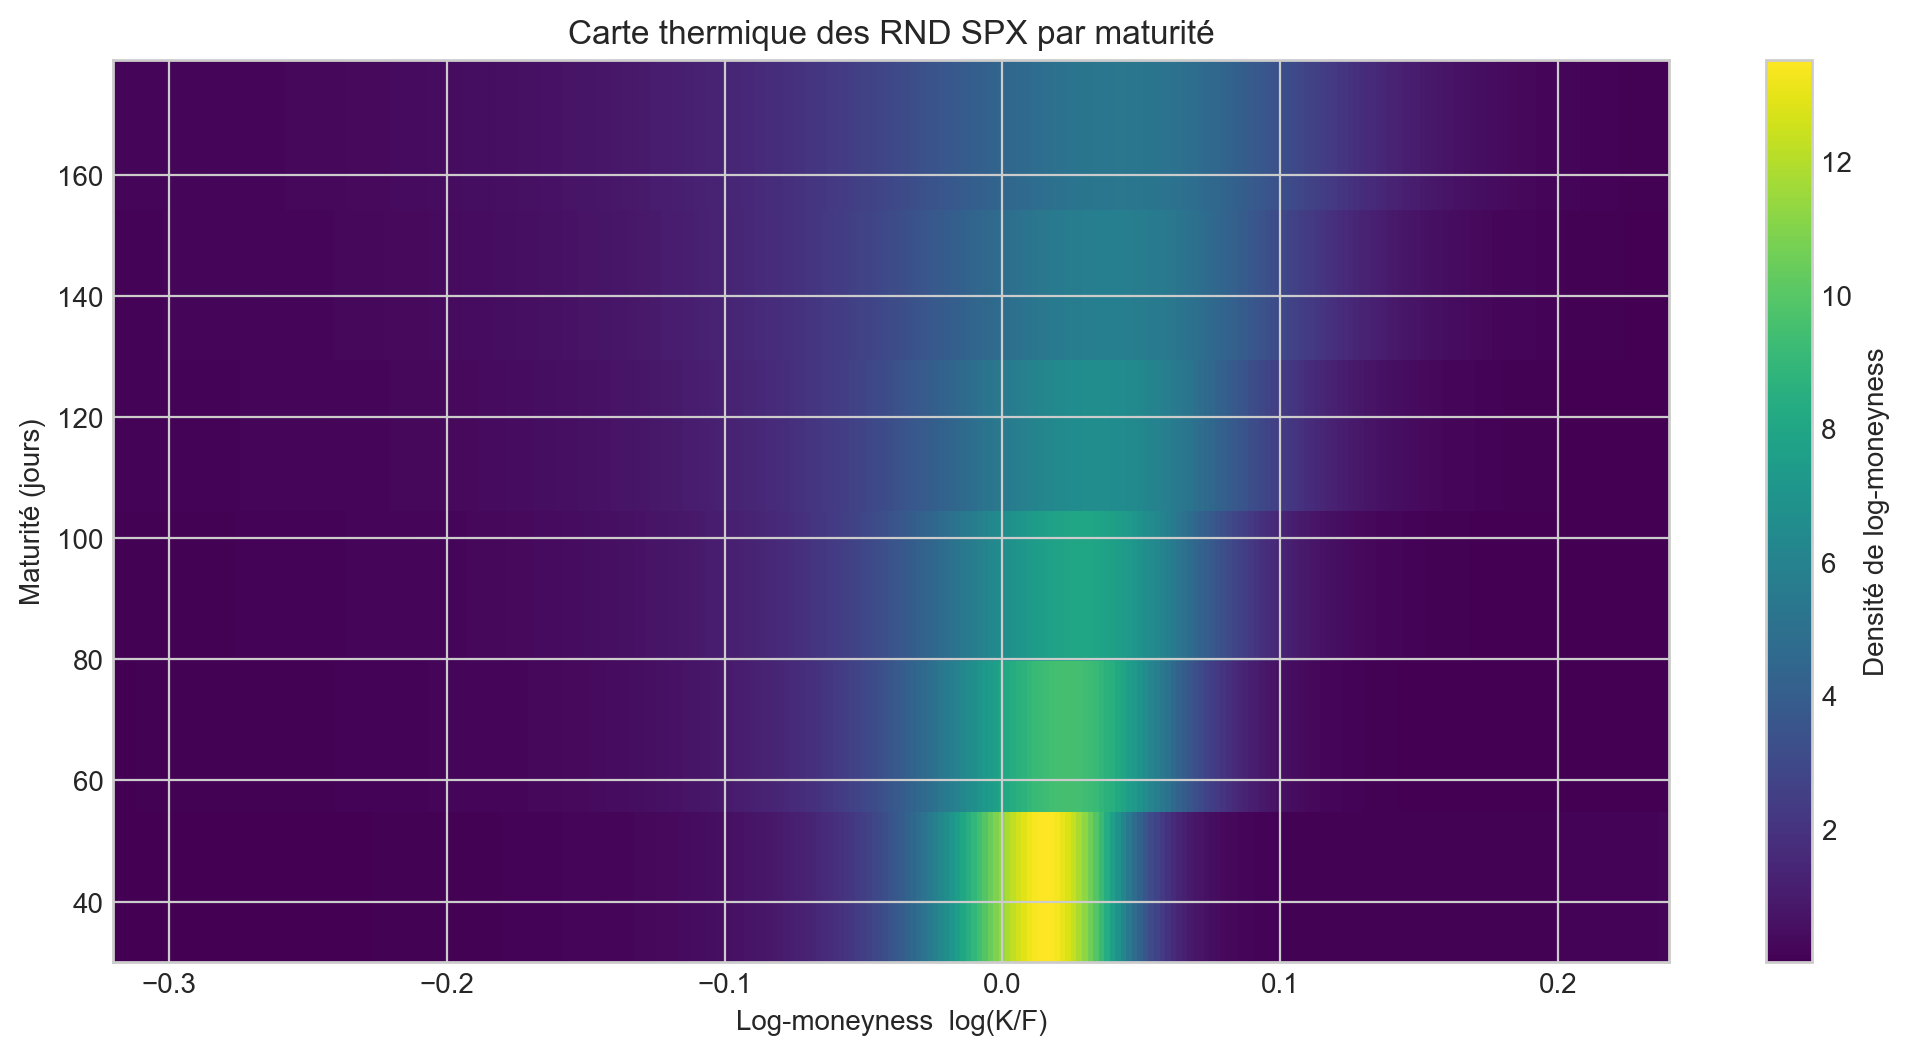
\includegraphics[width=0.92\textwidth]{results/06_rnd_heatmap_maturity.png}
\caption{Carte thermique des densités en log-moneyness.}
\end{figure}

\section{Validation informatique}
Le calcul de dérivée, masse, normalisation et moments est réimplémenté en Julia
1.10.10 sans package externe. L'écart absolu moyen avec Python est $3,3\times10^{-9}$
et l'écart maximal $2,1\times10^{-6}$, localisé aux bords de la grille.

\section{Vers une dynamique temporelle}
Avec un historique quotidien, chaque date produira une densité à horizon constant.
Les densités seront placées sur une grille commune, puis réduites par analyse
factorielle fonctionnelle. Les scores pourront suivre un AR ou un VAR. Les prévisions
seront comparées à une marche aléatoire fonctionnelle, c'est-à-dire la densité du jour
précédent. Les mesures incluront KL, Jensen--Shannon, Wasserstein et erreur de pricing.

La surface cible du projet aura alors pour axes date, log-moneyness et densité. Elle
ne doit pas être confondue avec la surface par maturité présentée dans cet article.

\section{Application future à la couverture}
Nous comparerons une couverture fondée sur la RND courante, une couverture utilisant
la RND prévue et un benchmark Black--Scholes. Les critères seront l'erreur de
couverture, sa variance, le drawdown et les coûts de transaction. L'incertitude de
prévision devra limiter l'agressivité des positions.

\section{Limites}
L'étude repose encore sur une seule date. Le seuil de spread est provisoire. La SVI
brute n'impose pas toutes les contraintes d'arbitrage butterfly. La surface 3D
interpole seulement six maturités. Enfin, l'absence d'un historique empêche pour le
moment toute conclusion sur la stabilité ou le pouvoir prédictif des RND.

\section{Conclusion}
Le premier prototype relie une chaîne SPX réelle à une densité contrôlée et
reproductible. Les résultats Python et Julia concordent. L'extension à six maturités
offre une première représentation tridimensionnelle économiquement interprétable.
Le prochain jalon essentiel est l'acquisition d'un historique quotidien permettant
de remplacer l'axe de maturité par un axe temporel et d'estimer les facteurs dynamiques.

\appendix
\section{Reproductibilité}
Le dépôt contient les snapshots bruts, tables nettoyées, scripts Python et Julia,
diagnostics, figures et commandes d'exécution. Le script principal est
\texttt{run\_prototype.ps1}. La surface 3D est produite par
\texttt{src/rnd\_surface\_3d.py}.

\printbibliography
\end{document}
